\documentclass[final]{siamart0516}

%% ------------------------------------------------------------------
%% Code used in examples, needed to reproduce 
%% ------------------------------------------------------------------
%% Used for \set, used in an example below
\usepackage{braket,amsfonts}
\usepackage{array}
%% Used for PgfPlots example, shown in the "Figures" section below.
\usepackage{pgfplots}
%% Used in table and figure examples below
\usepackage[caption=false]{subfig}
\usepackage{tablefootnote}

%% Used for creating new theorems, remarks
\newsiamthm{claim}{Claim}
\newsiamremark{rem}{Remark}
\newsiamremark{expl}{Example}
\newsiamremark{hypothesis}{Hypothesis}
\crefname{hypothesis}{Hypothesis}{Hypotheses}

%% Algorithm style, could alternatively use algpseudocode
\usepackage{algorithmic}

%% For figures
\usepackage{graphicx,epstopdf}
\usepackage{float}


%% For referencing line numbers
\Crefname{ALC@unique}{Line}{Lines}

%% For creating math operators
\usepackage{amsopn}
\DeclareMathOperator{\Range}{Range}

%% ------------------------------------------------------------------
%% End Code used in examples, needed to reproduce 
%% ------------------------------------------------------------------



%% ------------------------------------------------------------------
%% Begin User Defined Macros
%% ------------------------------------------------------------------
\newcommand{\cN}{\mathcal{N}}
\newcommand{\cL}{\mathcal{L}}
\newcommand{\aab}{\mathfrak{a}}
\newcommand{\one}{\mathbf{1}}
\newcommand{\zero}{\mathbf{0}}
\newcommand{\Jk}{\mathsf{J}}
\newcommand{\Jp}{\mathsf{J}_{\rm p}}
\newcommand{\Jl}{\mathsf{J}_{\rm ls}}
\newcommand{\Jat}{\mathsf{J}_{\rm at}}
\newcommand{\Jg}{\mathsf{J}_{\rm gl}}
\newcommand{\Pp}{\mathbb{P}_{\rm p}}
\newcommand{\Pl}{\mathbb{P}_{\rm ls}}
\newcommand{\Pg}{\mathbb{P}_{\rm gl}}
\newcommand{\Pat}{\mathbb{P}_{\rm at}}
\newcommand{\Phip}{\Phi_{\rm p}}
\newcommand{\Phil}{\Phi_{\rm ls}}
\newcommand{\Phig}{\Phi_{\rm gl}}
\newcommand{\Phia}{\Phi_{\rm at}}
\newcommand{\mup}{\mu_{\rm p}}
\newcommand{\mul}{\mu_{\rm ls}}
\newcommand{\mug}{\mu_{\rm gl}}
\newcommand{\nup}{\nu_{\rm p}}
\newcommand{\nul}{\nu_{\rm ls}}
\newcommand{\nug}{\nu_{\rm gl}}
\newcommand{\muat}{\mu_{\rm at}}
\newcommand{\nuat}{\nu_{\rm at}}
\newcommand{\nyst}{Nystr\"{o}m }

\definecolor{darkred}{rgb}{0.6,0.1,0.1}
\definecolor{darkgreen}{rgb}{0.1,0.6,0.1}
\definecolor{darkblue}{rgb}{0.1,0.1,0.6}
\def\as#1{\textbf{\textcolor{darkgreen}{#1}}}
\def\kl#1{\textbf{\textcolor{darkred}{#1}}}
\def\mi#1{\textbf{\textcolor{darkblue}{#1}}}


\newcommand{\GL}{\mathsf{GL}}
\newcommand{\Se}{S_{\epsilon}}
\newcommand{\We}{W_{\epsilon}}
\newcommand{\muy}{\mu^y}
\newcommand{\cF}{\mathcal{F}}
\newcommand{\ud}{u^{\dagger}}
\newcommand{\gt}{\rightarrow}
\renewcommand{\O}{\mathcal{O}}
\newcommand{\R}{\mathbb{R}}
\newcommand{\bbE}{\mathbb{E}}
\newcommand{\Q}{\mathbb{Q}}
\newcommand{\bbR}{\mathbb{R}}
\newcommand{\bbP}{\mathbb{P}}
\newcommand{\bbI}{\mathbb{I}}
\newcommand{\PP}{\mathbb{P}}
\newcommand{\C}{\mathcal{C}}
\newcommand{\G}{\mathcal{G}}
\newcommand{\B}{\mathcal{B}}
\newcommand{\BB}{\mathscr{B}}
\newcommand{\N}{\mathcal{N}}
\newcommand{\T}{\mathcal{T}}
\newcommand{\K}{\mathcal{K}}
\newcommand{\RR}{\mathcal{R}}
\newcommand{\M}{\mathcal{M}}
\newcommand{\HH}{\mathcal{H}}
\newcommand{\VE}{\varepsilon}
\newcommand{\dd}{ \,\textrm{d}}
\newcommand{\PAR}[1]{\partial #1}
\newcommand{\OL}[1]{\overline{#1}}
\newcommand{\EMPTY}{\varnothing}
\newcommand{\be}{\begin{equation}}
\newcommand{\en}{\end{equation}}
%% ------------------------------------------------------------------
%% End User Defined Macros
%% ------------------------------------------------------------------



\newcommand{\modas}[1]{\textcolor{magenta}{#1}\index {#1}}
\newcommand{\modk}[1]{\textcolor{blue}{#1}\index {#1}}
\newcommand{\modm}[1]{\textcolor{red}{#1}\index {#1}}
\newcommand{\modab}[1]{\textcolor{orange}{#1}\index {#1}}




%% ------------------------------------------------------------------
%% HEADER
%% ------------------------------------------------------------------

\title{Notes on Graph UQ Scaling}

%% ------------------------------------------------------------------
%% END HEADER
%% ------------------------------------------------------------------

%% ------------------------------------------------------------------
%% MAIN Document
%% ------------------------------------------------------------------
\begin{document}
\maketitle

\begin{abstract}
The purpose of this paper is to investigate the scaling of pCN and Gibbs sampler with respect to the number of data points under the assumption that the data points are sampled i.i.d from a fixed distribution $\bbP(X)$.  The problem has both a continuum and a discrete version. On the discrete side, one could study scaling limits.  On the continuum side, we can 1) formulate the continuum problem under $N\rightarrow \infty$, and $\epsilon \rightarrow 0$.  2) Study/prove whether pCN or Gibbs is well-defined in the limit. 
\end{abstract}

\section{Introduction}
% 1. Introduce the basic problem, and algorithms used to sample. 
% 2. Investigate the "performance" of these algorithm under large N, and different values of gamma. Since data points are sampled, could be considered discretizations of a continuum problem. And methods well-defined on the continuum will behave independent of the discretization size. 
% 4. To have a consistency in the $N$ large limit, we need to scale the precision matrix. Follow scaling in Slepcev, continuum Bayesian problem. 
% 5. Why spectral truncation is important? 
% 5. State our contributions.
%	a) methods well-defined on continuum? If not how? 
%	b) estimates for msj and acc? on continuum
%	c) empirical study of scaling with respect to N, as well as comparison between different methods, 
% 6. Define the methods here.   

Graph semi-supervised learning has many applications xxx. We state the problem setting for graph SSL. Let $Z = \{1\dots N\}$, and $Z' \subset Z$. $\{Y_j \in \{-1, 1\} | j\in Z'\}$ be the labels. The task is to infer the missing labels via the graph Laplacian $L$.  The optimization approach is to minimize a data fidelity term with regularization by q quadratic form $\langle u, Lu,\rangle$. 

In \cite{xxx}, this problem was formulated as a Bayesian inference problem, where the prior is a Gaussian $\cN(0, C)$.  Given some likelihood function $exp(-\Phi(u; y, \theta))$, we can form the joint probability distribution as 
$ \bbP(u|y) \propto exp(-J(u))$, where $$J(u) = \frac{1}{2}\langle u, Pu \rangle +\sum_{j\in Z'}\Phi(u(j); y(j), \theta).$$ In\cite{graphuq}, the authors sampled the posterior distribution to compute quantities that reflect the uncertainty of the prediction and the system. The algorithm used was pCN, an MCMC algorithm designed for Bayesian inverse problems that scales well with dimensionality. The Auxiliary variable Gibbs method is a popular alternative used in \cite{xxx} when the likelihood is probit. The goal of this paper is to study the scaling of these algorithms as $N\rightarrow \infty$, both theoretically and empirically. We need to specify how the feature vectors are obtained as the total number of points $N$ large.  the convention in \cite{xxx} and assume the points $\{x_i\}$ are sampled iid from some distribution $\rho$ supported on the domain $D$. We follow \cite{xxx} and assume the fidelity $Z'$ is finite.  Moreover, to simplify the analysis, we assume the first $J$ points of the i.i.d. samples $\{x_1, \dots, x_J\}$ are the fidelity samples. 

In order to have a consistent limit, we need to scale the graph Laplacian.  We also scale the in \cite{trillos2016variational}, so that the limiting dirichlet functional gamma converges to $\langle u, \cL u \rangle$, where $\cL$ is a diffusion operator. The reason for choosing this scaling is that  due to locality, the eigenvalues have asymtotic growth $O(j^{-d/2})$. Thus we can define a continuum Gaussian measure $\mu = N(0, (1 + \cL)^{-\alpha} )$, and define a continuum version of the problem. 
In particular, if the eigenfunctions and eigenvalues of the continuous Laplacian operator satisfy 
\begin{itemize}
\item $\lambda_k$ has growth $N^{\frac{d}{2}}$
\item Eigenfunctions $\phi_k$ are smooth up to boundary. 
\item $\sum_k k^{-\frac{\alpha d}{2}}\|\phi_k\|_\infty < \infty$. 
\end{itemize}
\modm{(Andrew: Refer to pdeML paper for references on the exact assumptions made on the spectrum and eigenvalues, and how they are reasonable if $\rho$ is smooth etc. )} The Gaussian is defined on the space of continuous function, and it is meaningful to evaluate $u$ at the fidelity points. 


We would hope that  $\mu^N$ approximates $\mu$ meaningfully. However, due to the fact that the eigenvectors of the Graph Laplacian converges at different rates, the full operator doesn't necessarily converge, as shown in the numerical experiments. 
Instead, we separate the limits, and define $\mu_{NK}$ and $\mu_K$ independently.  Namely, we approximate $\mu$ in two different limits. We call 

Our contribution in this paper is listed below:
\begin{enumerate}
\item we study the discrete approximations to the continuum. 
\item we prove a bound on pCN..
\item We study variations of the Gibbs method. 
\item Numerical Experiments. 
\end{enumerate}

Finally, some important notations are listed below. 
\begin{itemize}
\item $\mu_N, \mu$: The Gaussian prior on $\mathbb{R}^N$ and on the continuum $H^t$.
\item $\mu^N_K$, $\mu_K$: The degenerate measure induced by truncating the spectrum up to level $K$. 
\item $\pi_N, \pi$: The posterior. Assuming the $\pi \ll \mu$ and  $\pi_N  \ll \mu^N_0$. 
\item $\eta$ as the joint probability of $u, v$ under the posterior and the proposal $\bbP(v|u)$. 
\item $D$: The compact domain in $\mathbb{R}^N$ on which the density function $\rho$ is supported. 
\item $C$: The set on which the labels $y$ are observed. 
\end{itemize}


\section{Discrete Approximation}
% 1. To estimate quantities, we need to link discrete mu_N to mu. We use the tool in Slepcev in the spectral basis. 
% 2. mu_N does not actually approximate mu that well(see numerics) due to "slow" convergence of eigenvalues. Consider mu_{NK} and mu_K
% 3. Need Estimates on fixed nodes. Introduce the lemmas on restriction to a finite set of nodes, and corresponding corollaries. 

To study precisely the discretization error from $\mu_{NK}$ to $\mu_K$, we need study the measures from the perspective of the eigenfunctions $q_k$ and $q_k^N$ via the $KL$ expansion. For notational simplicity, we assume that the spectrum of the continuous operator $L$ has distinct eigenvalues. However it is straightforward to generalize to the general case. We summarize the convergence analysis Slepcev 17 in Proposition 1, which is proved in the appendix. 
\begin{proposition}
Let $\rho$ be the density function defined on the domain $D$.  Let $\cL$ be the continuous Laplacian operator,  $\lambda_1 < \lambda_k$ be eigenvalues of $\cL$, and $q_k$ be the eigenvectors of $\cL$.    Given $\omega = \{x_i\}$ is a sequence of i.i.d. sample from $\rho$, we can define the discrete graph Laplacian as $s_n L_n$. We denote $\lambda_{NK}$ as the discrete eigenvalues, and $q_k^N$, a choice of the eigenvectors corresponding to $\lambda_{NK}$.  Then for any fixed $K$, the following holds almost surely with respect to $\omega$. 
\begin{enumerate}
\item $\lim_{N\rightarrow \infty} \lambda_{NK} = \lambda_K$
\item There exists a choice of eigenvectors $\{q_{NK}\}$  for each $N$ such that $$\lim_{N\rightarrow \infty}\|q_{NK} - \pi_N(q_{K})\|_{\nu_N} \rightarrow 0$$
\end{enumerate} 
\end{proposition}

We apply proposition 1 to prove the convergence of expectations for a class of functionals $F_N$ and $F$.  Namely, we want them to satisfy the continuity condition 
\begin{definition}
Suppose $F_N$ be functionals defined on $u\in \mathbb{R}^N$, and $F$ be functionals on $u\in \mathbb{R}^N$. We say $F_N$ and $F$ satisfy the continuity condition if$\|u_n - \pi_n(u) \|_{\nu_n} = 0$ implies $F(u) = F_N(u)$.  
\end{definition}
\begin{proposition}
Let the variables and notations be the same as in Proposition 1, and $F_N$, $F$ are functional defined in 2 satisfying the continuity condition. If $F_N$ and $F$ are bounded, then $$\lim_{N\rightarrow \infty} \bbE_{\mu_{NK}} F_N  = \bbE_{\mu_{K}} F$$
\end{proposition}
\begin{proof}
Given the choice of basis $q_k$, we can express the expectations in terms of the eigenbasis $q^k$. $E(F) = \int exp(-\| \xi \|^2) G_N(\xi)$. Since $q_{NK}$ and $q_K$ are close, $G_N$ converges to $G$ point-wise. By dominated convergence, we have $E_{NK}$ converges to $E_K$. 
\end{proof}

Since the likelihood is defined on the set of fidelity points, We need to control $q_{NK}$ and $q_K$ on the set of fidelity points. To avoid $L^\infty$ estimates, we make the assumption that the labels are given on the first $J$ samples of $x$. 
 
\begin{proposition}
Let $q^k$ be the continuous eigenvectors. For all $k$ and $\epsilon > 0$, we have with probability $1 - o(1)$ that $\exists \{q_{NK}\}$ eigenvectors of $L_N$ such that $\|\pi^N_J(q_{NK}) - \pi_J(q_K)\|_\infty < \epsilon$. 
\end{proposition}
\begin{proof}55qzyu 

\end{proof}

As an immediate corollary, we show the restriction of the measures on a finite fidelity set are close. 
\begin{corollary}
Let $\mu^J_K:= \pi_J^*(\mu_K)$, and $\mu^J_{NK}:=\pi_J^*(\mu_{NK})$. Let $C_{NK}^J$ and $C_K^J$ be the covariance matrix of these Gaussian measures on $\mathbb{R}^J$.   For all $k$ and $\epsilon > 0$, we have with probability $1 - o(1)$  that $\|C_K^J - C_{NK}^J\| < \epsilon$. 
\end{corollary}



\section{Analysis of pCN}
% 1. Well-defined on continuum, and cite results. 
% 2. Prove bounds on acc and msj for mu_K and mu. 
% 3. Show discrete difference is small. 
Given a Gaussian measure, the the pCN algorithm stated below:
\begin{align}
\begin{aligned}
v &= (1 - \beta^2)^{\frac{1}{2}}u + \beta w\\
a(u,v) &= exp(\Phi(u) - \Phi(v))
\end{aligned}
\end{align}
pCN is well defined in the continuum, as well as on the truncated space $\mu_{K}$ and the diffuse limit theory in \cite{pillai2011random} is applicable. 

In this paper, we use basic calculations to show that the expected acceptance probability and mean square jump have a non-zero upper bound on the continuum problem, and show this bound holds under the truncation error and the discretization error is small. 

We first prove a bound on the acceptance probability of the pCN method. The quantity $Z = \int_{u} \one_A(u) d\mu_J(u) = \int_{u} \one_A(u) d\mu(u)$ needs to be positive to ensure the existence of a conditional probability, and positivity. We assume that the label set $y$ is chosen such that $Z$ is positive. We call such assignments a \emph{compatible} label assignment. 


\begin{proposition}
Let $u \sim \mu_p$ the posterior, and $v$ according to the pCN proposal. Suppose the log likelihood $\Phi$ satisfies $0<\Phi(u; y) <C$ if $Sign(u) = y$. Then we have the estimate
$$\bbE_{\mu_p} a(u, v) \geq \frac{Z}{C}$$ where $A = \{u | Sign(u) = y\}$,  $Z = \int_{u} \one_A(u) d\mu_J(u) = \int_{u} \one_A(u) d\mu(u)$
\end{proposition}
\modm{(Check the constants more carefully and make sure they are in [0, 1])}
\begin{proof}
 
\begin{align}
\begin{aligned}
\bbE_{\mu_p} a(u, v) &= \int_u ( \int_v exp(\Phi(u) - \Phi(v)) d\bbP(v|u)) d\mu_p(u) \\
&\geq  \frac{1}{C}\int_u ( \one_A(v) d\eta_u(v)) d\mu_p(u) = \frac{1}{CZ'} \int_u ( ( \one_A(v) d\eta_u(v))) \one_A(u)d\mu(u) 
\end{aligned}
\end{align}
Where $Z' = \int_{u} exp(-\Phi(u)) d\mu(u) \geq \int_{u} \one_A(u) d\mu_J(u)$. 
Note that the integrant function factors through the projection $\pi_J$, 
\begin{align}
\begin{aligned}
\int_u ( \bbP(v\in A|u)) \one_A(u)d\mu(u) &= \int_{u} \bbP(v>0|u) \one_A(u) d\mu_J(u) \\
&= \int_{u} (\int_{w} \one_A(w  +\frac{\sqrt{1 - \beta^2}}{\beta} u) d\mu_J(w)) \one_A(u) d\mu_J(u)\\
&\geq \int_{u} (\int_{w} \one_A(w) d\mu_J(w)) \one_A(u) d\mu_J(u)\\
&=(\int_{u} \one_A(u) d\mu_J(u))^2
\end{aligned}
\end{align}
\end{proof}
Since the analysis holds regardless of the Gaussian measure and the space it was defined on, the same estimates holds if we replace $\mu$ with $\mu_{NK}$ and $\mu_K$. Hence to prove an upper bound for the discrete and continuous truncated measure, we need to show the quantity $Z$ is close to $Z_{NK}$ and $Z_K$. 

\begin{proposition}
Let $Z_K = \int_{u} exp(-\Phi(u)) d\mu_K(u) = \int_{u} exp(-\Phi(u)) d\mu_K^J(u)$. Then $\lim_{K\rightarrow \infty} Z_K = Z$. 
\end{proposition}
\begin{proof}
This comes from the fact that $\mu$ is trace class, and hence $\mu_K^J$ converges to $\mu^J$. 
\end{proof}
For the discrete approximation, we have 
\begin{proposition}
Let $Z_{NK} = \int_{u} exp(-\Phi(u)) d\mu_K(u) = \int_{u} exp(-\Phi(u)) d\mu_{NK}^J(u)$. Then for all $\epsilon > 0$, with probability $1 - o(1)$, $|Z_{NK} - Z_K| < \epsilon$. 
\end{proposition}
\begin{proof}
Since $|\mu_{NK}^J - \mu_{K}^J\| < \epsilon$, we have $Z_{NK}$ and $Z_K$ are close with probability $1 - o(1)$. 
\end{proof}

We prove an estimate for the mean square jump as well. 
\begin{proposition}
Define the mean square jump as $\bbE_{\mu_p} \|u - v\|^2$. Then for $0 < \Phi(u; y) < C$ for $S(u) = y$, we have  $\bbE_{\mu_p} \|u - v\|^2 > C'$ for some positive constant $C'$ independent of $beta$, $\Phi$. 
\end{proposition}

\begin{proof}
\begin{align}
\begin{aligned}
\bbE_{\mu_p} \|u - v\|^2 &= \int_u ( \int_{v\in A} \|u - v\|^2 d\bbP_{v|u}) d\mu_p(u)\\
&=  \int_u ( \int_{v} \|u - v\|^2 \one_A(v) \bbP_{v|u} ) \one_A(u) d\mu(u) \\
&= \int_u ( \int_{v} \|\beta w - \beta' u\|^2 \one_A(w  +\frac{\sqrt{1 - \beta^2}}{\beta} u) d\mu(w) ) \one_A(u) d\mu(u)\\
&\geq \int_u ( \int_{w} \|\beta w - \beta' u\|^2 \one_A(w) d\mu(w) ) \one_A(u)  d\mu(u) \\
&\geq \beta^2 \int_u( \int_{w} \|w - \frac{\beta'}{\beta} u\|^2 \one_A(w) d\mu(w)) \one_A(u) \one_{\|u\| \geq 2\delta} d\mu(u) \\ 
&\geq \beta^2 \int_u( \int_{w} \|w - \frac{\beta'}{\beta} u\|^2 \one_A(w) \one_{\|w\| \leq \delta} d\mu(w)) \one_A(u) \one_{\|u\| \geq 2\delta} d\mu(u) \\
&\geq \delta^2 \beta^2 \int_u( \int_{w} \one_A(w) \one_{\|w\| \leq \delta} d\mu(w)) \one_A(u) \one_{\|u\| \geq 2\delta} d\mu(u) \\
&= \delta^2 \beta^2 ( \int_{w} \one_A(w) \one_{\|w\| \leq \delta} d\mu(w)) \times (\one_A(u) \one_{\|u\| \geq 2\delta} d\mu(u) )
\end{aligned}
\end{align}

where $\beta' = 1 - \sqrt{1 - \beta^2}$, and $\delta > 0$. 
Hence we have to show that for $\delta > 0$,   $ \int_{w} \one_A(w) \one_{\|w\| \leq \delta} d\mu(w)$ and $\int_u \one_A(u) \one_{\|u\| \geq 2\delta} d\mu(u)$ are both greater than $0$. 
\end{proof}
We show this bound is stable under truncation and discretization.
\begin{proposition}
Let $I = \int_{w} \one_A(w) \one_{\|w\| \leq \delta} d\mu$. Then $\lim_{K \rightarrow \infty} I_K = I$. 
\end{proposition}
\begin{proof}
Cite standard theory for weak convergence of measures $\mu_K$ to $\mu$?
\end{proof}
\begin{proposition}
Let $I_K = \int_{w} \one_A(w) \one_{\|w\| \leq \delta} d\mu_K$, and $I_{NK} =  \int_{w} \one_A(w) \one_{\|w\| \leq \delta} d\mu_{NK}$, Then $|I_K - I_{NK}| < \epsilon$ with probability $1 - o(1)$. 
\end{proposition}
\begin{proof}
We use Proposition 2. Under such a basis $q_{NK}$, we have 
$$I_{NK} = \int \one_A(Q^J_N \xi) \one_{B_\delta}(\xi) exp(-\|\xi\|^2_{\Lambda_N}) d\xi$$. 
By convergene of eigenvalues $|I_{NK} - I_K| < \epsilon$. 
\end{proof}


\section{Auxilary Variable Methods}
% 1. Show GibbsI method "freezes" for $k$. 
% 2. Gibbs II well-defined on continuum. Show estimates for $Gamma$ small
% 3. HH well-defined, designed to combat large correlation for small gamma. Key difference is integrating out $u$. In small gamma limit, equivalent to restriction on nodes. P(u1|y) and P(u2|u1). Dependes on how P(u1|y) is sampled. Show pCN on P(u1|y) then P(u2|u1) is equivalent to P(u|y). 
 
\subsection{Gibbs Method}
The Auxilary variable Gibbs approach is to model the variable $u^*(j) = u(j) + \epsilon$. There are two ways. One is to model $u^*$ on all nodes, the second is to only model $u^*$ on labelled nodes. We call these two approach Gibbs(I) and Gibbs(II). We show Gibbs(I) does not scale well with $N$. 

\begin{align*}
&P'=P+\gamma^{-2}I,\\
&P'm=\gamma^{-2}u^*.
\end{align*}


The Standard Gibbs method(I) is ill defined on the continuum. This should reflect in the slowing down of Gibbs sampler as $N\rightarrow \infty$.  This should be similar to \cite{agapiou2014analysis, beskos2009optimal}. 
We quantify this slowing down precisely in the next proposition. 

\begin{proposition}
Given fixed $u$, let $u^+$ be the value of the next sample. Let $\hat{u}^*_k = \langle u^* , q_{NK} \rangle$. Then $\hat{u}^+_k = \hat{u}_k(1 + o(1))$ with large probability. 
\end{proposition}
\modm{(Andrew: Formulate this more elegantly as the ``white noise disappearance problem" in the continuum. }
%\begin{align}
%\begin{aligned}
%\hat{u}^*_k &= \hat{u}_k + \xi_k\\
%\hat{u}^+_k &= (1 + \frac{\lambda^k_N}{N})^{-1}(\hat{u}_k + \xi_k) + \eta_k(1 + \frac{\lambda^k_N}{N})^{-1/2}
%\end{aligned}
%\end{align}
%If $N\gg J$, $\xi_k$ will be almost $N(0, 1)$ by law of large numbers, and $\lambda^k_N/N$ will be $O(1/N)$. Hence the Gibbs sampler is maximally correlated on the first few components of the Fourier basis. 

Let $u^*(j)=u(j)+\eta(j), j \in Z'$ be only on the fidelity set. Then $\bbP(u^*|u,y)$ as before is independent truncated Gaussians. 
$\bbP(u|u^*,y) = N(m, P')$, where 
\begin{align*}
&P'=P+\gamma^{-2}D_J,\\
&P'm=\gamma^{-2}E_Ju^*, 
\end{align*}
where $I_J = [I_J, 0; 0, 0]$, and $E_J = [I_J; 0]$. 


Standard Gibbs method(II) seems well-defined on the continuum, and empirically behaves well when $N$ large. However, when $\gamma$ is small, the method freezes on the observed labels $\{x_1, \dots x_J\}$. 
\begin{proposition}
Let $u \in \mathbb{R}^N$. Then $\|u^+_J - u_J\|_\infty \leq \gamma \|u_J\|_\infty$. 
\end{proposition}

\subsection{Holmes and Held}
In Holmes and Held, the standard Gibbs method was revised to handle the case of small noise $\gamma$, by considering the factorization $\bbP(u, u^* |y) = \bbP(u*|y)\bbP(u|u^*)$. The method first samples from $\bbP(u^*|y)$, and then samples $u$ according to $\bbP(u|u^*)$, which is a Gaussian. 

To study Holmes and Held, and compare with other methods, it is necessary to list two key components of this method. The first is the auxilary variable approach, to sample $\bbP(u, u*|y)$ jointly. This is the same with the Gibbs sampler.  The second idea which is the key for small $\gamma$ is to marginalize $u$ and sample from $\bbP(u^*|y)$. 

Since the HH methods is designed for small $\gamma$, it is telling to study the algorithm in the small $\gamma$ limit. 
In the small $\gamma$ limit, HH reduces to sampling $\bbP(u_1|y)$, and then sampling $\bbP(u_2|u_1)$, where $u = (u_1, u_2)$, where $u_1$ is the value of $u$ on the observed nodes.  The efficacy of the algorithm depends on the sampler used for $\bbP(u1|y)$. In fact, one can use pCN to sample from $\bbP(u1|y)$. The proposition below shows a connection between the pCN method, and HH-pCN.

\begin{proposition}
Let $u = (u_1, u_2)$. Suppose $v = (v_1, v_2)$ the proposal from pCN, $w = (w_1, w_2)$ be from the HH-pCN method, and $acc_1(u, v)$, $acc_2(u,w)$ be the corresponding acceptance probabilities. Then $acc_1 = acc_2$ as a function of $(u,v)$, $w_1 = v_1$ in law. Moreover, $w_1 = (1 - \beta) xxx w_2$ in law. 
\end{proposition}

\begin{proof}

\end{proof}



%\begin{itemize}
%\item sample $v$ from $\bbP(v|y) \propto N(0, P'') \Pi_{j\in Z'}Ind(S(v_j) = y_j)$ via some component-wise Gibbs sampler.  $P'' = (\gamma^{-2} I + \gamma^{-4}(P + \gamma^{-2})^{-1})$
%\item sample $u$ via $\bbP(u|v) = N(m, P')$, $m = \gamma^{-2} P'^{-1} v$ and $P' = P + \gamma^{-2} I$. 
%\end{itemize}




\section{Numerical Experiments}
% 1. Acc curve pCN, msj
% 2. auto/correlation time Mean Variance vs N pCN, Gibbs Holmes method
% 3. discrete spectrum. 
\subsection{Large $N$ limits of pCN, Gibbs}
This section studies the large $N$ behaviour of pCN and Gibbs (I) and (II). We sample $N = 2000:1000:8000$ samples from a uniform distribution on a square domain, and choose five points in the square as fidelity, with 2 points in class 1 and 3 points in class 2. We use the scaling in slepcev17 paper, and project to $60$ eigenvectors. We vary $\gamma = [0.1, 0.3, 0.7, 1.0]$ over a moderate range, and plot the acceptance probability (for pCN only), the mean square jump, the empirical $l2$ error over $2 \times 10^4$ iterations, as a function of $N$. Each experiment is averaged over $10$ realizations of samples from the uniform distribution.


\begin{figure}[!ht]
\centering
{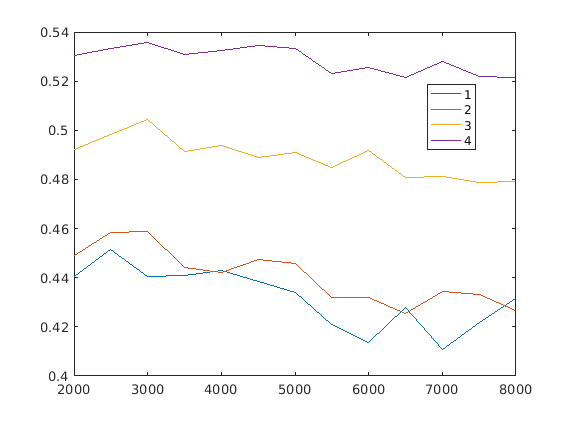
\includegraphics[width=80mm]{Figures/Convergence_accprob_pCN.png}}
\caption{acceptance probability of pCN}\label{fig:pcn-acc}
\end{figure}
 
\begin{figure}[!ht]
\centering
\subfloat[pCN]{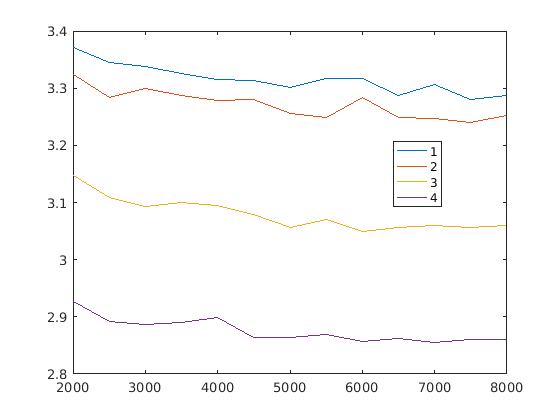
\includegraphics[width=50mm]{Figures/Convergence_msj_pCN.png}}
\subfloat[Gibbs I]{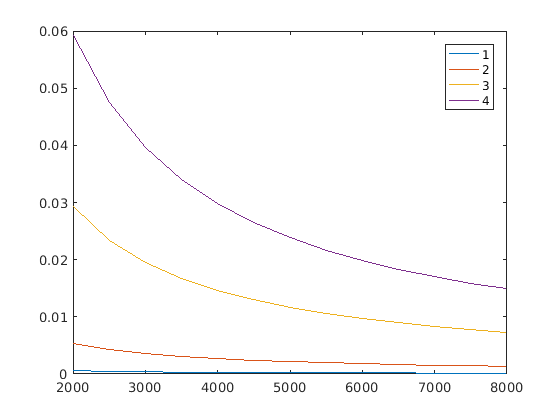
\includegraphics[width=50mm]{Figures/Convergence_msj_G1.png}}
\subfloat[Gibbs II]{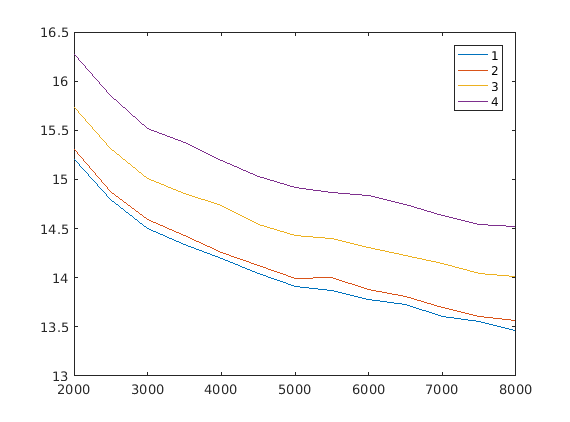
\includegraphics[width=50mm]{Figures/Convergence_msj_G2.png}}
\caption{Mean Square Jump}\label{fig:msj1}
\end{figure}
 

\begin{figure}[!ht]
\centering
\subfloat[pCN]{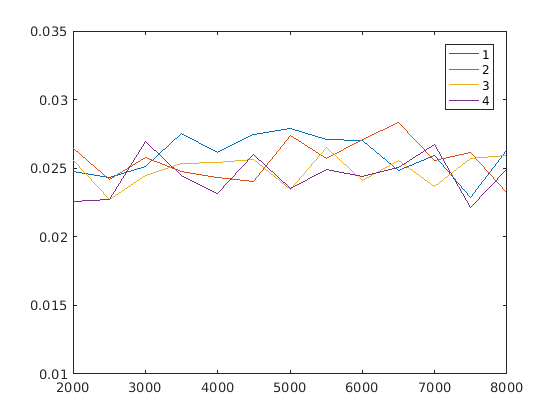
\includegraphics[width=50mm]{Figures/Convergence_uerr2_pCN.png}}
\subfloat[Gibbs I]{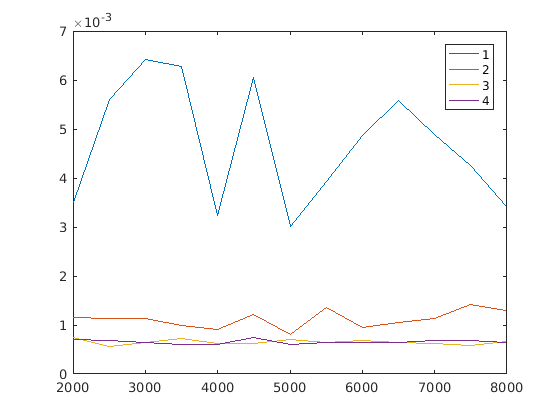
\includegraphics[width=50mm]{Figures/Convergence_uerr2_G1.png}}
\subfloat[Gibbs II]{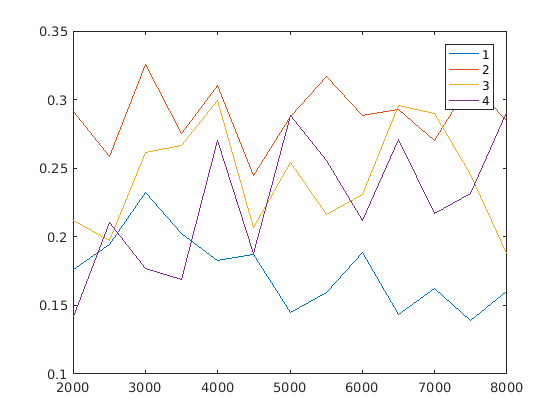
\includegraphics[width=50mm]{Figures/Convergence_uerr2_G2.png}}
\caption{$L2$ error}\label{fig:errl2}
\end{figure}

\subsection{Small $\gamma$ Limit}
This section compares the Gibbs sampler and the probit under the small $\gamma$ limit. We choose $\gamma = 1e-3$, and plot the sampled values of $u(j)$ for $j\in J$ in the fidelity set. We see the Gibbs(II) method freezes on those nodes, while the pCN method does not.

\begin{figure}[!ht]
\centering
\subfloat[pCN]{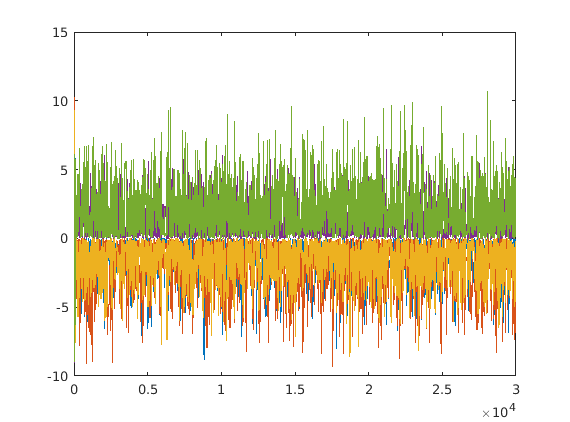
\includegraphics[width=50mm]{Figures/Convergence_smallgamma_uJ_pCN.png}}
\subfloat[Gibbs II]{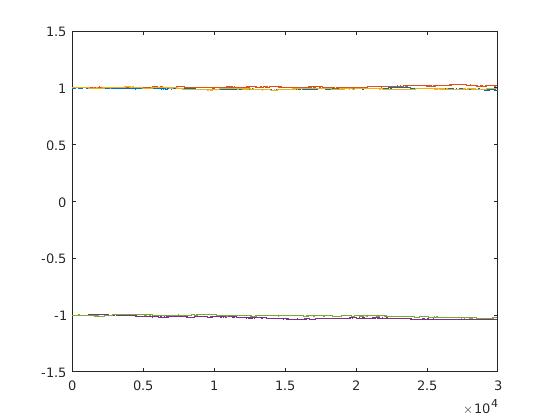
\includegraphics[width=50mm]{Figures/Convergence_smallgamma_uJ_G2.png}}
\caption{Samples of $u(j)$ for $j \in J$.}\label{fig:uj-smallgamma}
\end{figure}

\subsection{Gaussian measures}
In this section, we study the quality of the approximation of $\mu_N$, $\mu_{NK}$ to the continuum by studying the pushforward of these measures on a finite set of points. We demonstrate empirically that pushforward of the full discrete Gaussian measure $\mu_N$ does not converge the continuum measure $\mu$ when $N$ increases.  Moreover, we show that the truncated measure $\mu_{N,K}$ by choosing $K$ such that the spectrum as converged, approximates the true continuum $\mu$ better than the full Laplacian.

This shows empirically that the eigenvectors/values of $L_N$ which have not yet converged to the continuum induces a non-trivial error away from the true continuum limit.

\begin{figure}[!ht]
\centering
{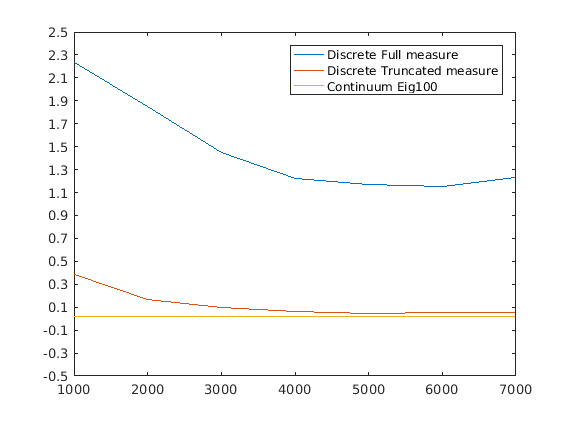
\includegraphics[width=80mm]{Figures/Pushforward.png}}
\caption{$l2$ err of Covariance matrix $C_{JJ}$ as a function of $N$ computed from $L_N$, $L_{NK}$ and the continuum measure $\mu$.}\label{fig:gaussian-pushforward}
\end{figure}
 

\appendix

\section{Gaussian measures}
We look at measures of the form $mu$ whose covariance operator is $C = (L + \tau I)^\alpha$ with $\alpha > 1$. From Slepcev17, we have that the eigenvalues and the eigenvector projections converge to its continuum limits. However, this convergence is not uniform among different eigenspace. In fact, we empirically observe that only a small fraction $K \ll N$ of the eigenvectors have actually converged. Moreover, the eigenvectors that have not converged can even hinder the convergence of certain quantities as $N\rightarrow \infty$. This motivates us to consider decoupling the number of nodes $N$ and the number of eigenvalues $K$, and study separate limits. 

\begin{itemize}
\item For fixed $K$, we show that for certain functions $f$, $|E_{\mu^N_k} f - E_{\mu_k}f|$ is small with high probability.
\item We show that for certain $f$, $|E_{\mu_k} f - E_{\mu_k}f|$ is small for large $k$. 
\end{itemize}
The second point follows from the fact that $\mu$ is trace class, while the first fact uses conclusions about the approximation of the continuum eigenvectors from the discrete. 

\subsection{Approximation of Eigenvectors}
We first prove a proposition which shows that we can approximate an orthonormal eigenbasis of the discrete Laplacian that spans $V_K^N$ by restricting a set of orthonormal eigenbasis in the continuous domain to the set of data points.  
\begin{proposition}
Let $V_k$ be the eigenspace of $L$ of the eigenvalue $\bar{\lambda}_k = \lambda_{\hat{k}}, \dots, = \lambda_{\hat{k} + s(k)}$. Let $\{v_j\}$ be eigenvectors of $L^n$ corresponding to the eigenvalues $\lambda_j^n$. Then almost surely, $\exists \{\phi_j^{(n)}\}$ an eigenbasis of $V_k$ such that $\lim_{n\rightarrow \infty}\|\tilde{\phi}_j^{(n)} - v_j\|_{\nu_n} = 0 $, where $\tilde{\phi}_j^{n} = \phi_j^{n}(x_1, \dots, x_n) \in \mathbb{R}^n$. 
\end{proposition}
\begin{proof}
Let $\{\phi^j\}$ be a choice of an eigenbasis of $V^k$, and $\phi_j^{n} = \phi_j(x_1, \dots, x_n)$. By smoothness of $\phi_j$, $\phi_j^{n} \rightarrow \phi_j$ in the $TL2$ sense. Let $w_j^n = Proj^N_K(\phi_j^{n})$, then $w_j^n \rightarrow Proj_k(\phi_j) = \phi_j$ in $TL2$.  Hence $\|w_i^n - \phi_i^n\|_{\nu_n} \rightarrow 0$. Moreover, $G_{ij} = \langle w_i^n, w_j^n \rangle_{\nu_n} \rightarrow \delta_{ij}$ as $n\rightarrow \infty$. Since $G$ is full rank, $\{w_j\}$ spans $V^n_k$. Let $\{w_j^{'n}\}$ be the Grahm-Schmidt orthogonalization of $\{w_j^n\}$. Note that if the Gram matrix $G$ is sufficiently close to the identity, $\|w_j^{'n} - w_j^n\|_{\nu_n}$ will be small.  Hence we can choose $N$ such that $\forall n > N$, $\|w_j^{'n} - w_j^n\|_{\nu_n} < \epsilon$, and $\|w_j^{'n} - \phi_j^n\| \leq 2\epsilon$. 

Let $Q$ be an orthogonal transform mapping $w_j^{'n}$ to $v_j^n$. Then letting $\phi'_j = \sum_i \phi_i q_{ij}$, we have $\|\phi_j^{'n} - v_j\| = O(\epsilon)$. 
\end{proof}

It is useful to study the convergence of the eigenfunctions when restricted to the first $J$ components. Since the convergence is in TL2, this does not follow immediately from the original theorem. However, we are able to prove: 

\begin{proposition}
Let $\{x_i\}$ be an i.i.d. sequence sampled from $\rho$.  Let $v_i^n$ be eigenvectors of $V^n_k$. Then with probability $1 - o(1)$ with respect to $N$, $\exists \phi_j$ such that $|\phi_i(x_j) - v^n_i(j)| < \epsilon, \quad \forall i = \{1, \dots, J\}, j = 1, \dots s(k)$. 
\end{proposition}
 
 
\begin{proof}

Let $E^J_{n, \epsilon}$ be the event $\{w = \{x_i\} | \exists \phi_j \quad \text{s.t. } |\phi_j(x_i) - v^n_i(j)| < \epsilon \}$. Since $\{x_i\}$ is i.i.d, $P(E^J_{n, \epsilon}) = P(E^{J'}_{n, \epsilon})$, $\forall |J'| = |J|, J' \subset \{1, \dots, n\}$. Let $dJ'$ be the uniform measure on subsets of size $|J|$, we have 
\begin{align}
\begin{aligned}
P(E^J_{n, \epsilon}) &= \int_{J'} \int_w \one_{E^{J'}_{n, \epsilon}}(w) dw dJ'\\
&= \int_{w} \int_{J'} \one_{E^{J'}_{n, \epsilon}}(w) dJ'dw 
\end{aligned}
\end{align}
Define the set $F_{n, \delta} = \{w| \exists \{\phi_j\}, \quad s.t.\quad \|\phi_j^n - v_j^n\|_{\nu_n} < \delta ,\forall k \leq K \}$. Note that if $\|\phi^n_j - v^n_j(i)\|_{\nu_N} < \delta$, then $|\phi^n_j(i) - v^n_j| < \epsilon$ for all $i$ except on a set $K(w)\subset \{1, \dots, n\}$, $|K(w)| <\frac{\delta}{\epsilon} n$. 
Hence 
\begin{align}
\begin{aligned}
 \int_{J'} \one_{E^{J'}_{n, \epsilon}}(w) dJ' &\geq  \int_{J'} \one_{F_{n, \delta}}(w) \one_{J' \cap K(w) = \emptyset}(J')dJ'
\end{aligned}
\end{align}
Therefore
\begin{align}
\begin{aligned}
P(E^J_n) &\geq \int_{w} \one_{F_{n, \delta}}(w) (\int_{J'} \one_{J' \cap K(w) = \emptyset}(J') dJ') dw\\
&= \int_{w}\one_{F_{n, \delta}}(w) \one_{J' \cap K(w) = \emptyset}(J') dJ'\\
&\geq \int_{w} \one_{F_{n, \delta}}(w) (1 - C\frac{\delta}{\epsilon})^J\\
&= P(F_{n, \delta})  (1 - C\frac{\delta}{\epsilon})^J
\end{aligned}
\end{align}
where the above holds for any $\delta$. We want to use the above to show $\lim_{n \rightarrow \infty}P(E^J_{n, \epsilon}) = 0$ by choosing a sequence of $\delta_n \rightarrow 0$. Note that from above, we have $P(\cap_\delta \cup_N \cap_{n>N} F_{n, \delta}) = 1$. Let $G_{N, \delta} = \cap_{n>N} F^{J}_{n, \delta}$. Note that $\lim_{N\rightarrow \infty} P(G_{N, \delta}) = 1$ monotonically, and $P(G_{N, \delta_1}) < P(G_{N, \delta_2})$ if $\delta_1 < \delta_2$.  Given any $\sigma$, we choose $\delta$ such that $(1 - C\frac{\delta}{\epsilon}) > (1 - \sigma/2)$, and $N$ such that $P(F_{n, \delta}) > 1 - \sigma/2$. Then $P(E^J_{n, \epsilon}) > 1 - \sigma$, $\forall n > N$. 
\end{proof} 
 
 
\subsection{Approximation of Gaussian Measures} 
We compare the Gaussian measures $\mu_K$ and $\mu_{NK}$. Since the two measures are not defined on the same space, we do not directly compare the two measures, but instead map these measures to the Fourier space. Namely, given an eigenbasis $\{\phi_j\}$, we can identify $R^K$ with $V^K$ via $\Phi: (\xi_1, \dots, \xi_k) \mapsto \sum_i \xi_i \phi^i$. Define $\tilde{\mu}_K = \Phi^{-1*} \mu_K$, we show in the proposition below that there exists an eigenbasis $\Phi$ such that $\tilde{C}_K \approx \tilde{C}_K^N$, and $\phi^n \approx v^n$.  

\begin{proposition}
Let $\phi_j$ be orthonormal basis of $V_K$. There almost surely exists an orthonormal basis $\{q^n_j\}$ of $V^N_K$ such the following holds: 
\begin{enumerate}
\item $q^n_j \rightarrow \phi_j$ in $TL2$. 
\item The measure $\tilde{\mu}_{NK} := Q^{-1*}(\mu_NK)$ defined on $\mathbb{R}^K$ converges to $\tilde{\mu}_{K} := N(0, C)$, where $C$ is the diagonal matrix. 
\end{enumerate}
\end{proposition}
\begin{proof}
(sketch): We show than under an orthonormal transform of the eigenbasis $v^n_j$ to $q^n_j$, we have $\|q^n_j - \phi^n_j\|_{\nu_n}\rightarrow 0$. Thus $q^n_j \rightarrow \phi_j$ in TL2. Moerover, since the transform preserves $V^K_N$, $|\tilde{mu}_{NK} - \tilde{\mu}_K| = o(1)$. 
\end{proof}
As a corollary, we can show that $\lim_{n\rightarrow \infty}E_{\mu_nk} f^n = E_{\mu_K} f$ almost surely for certain class of $f$. 
\begin{corollary}
Let $f^n$ be a bounded function defined on $\mathbb{R}^N$, $f$ such that $f^n(u^n) \rightarrow f(u)$ $\forall, u^n \rightarrow u$. Then $\lim_{n\rightarrow \infty}E_{\mu_{nk}} f^n = E_{\mu_K} f$
\end{corollary}
\begin{proof}
(sketch): Choose $\{q^n_j\}$ the basis as above. Let $g^n(\xi) = f(\xi^Tq^n)$. Then $g^n \rightarrow g$ point-wise by property of $f$. Since $\tilde{\mu}_{NK} \rightarrow \tilde{\mu}{K}$, by dominated convergence, $E_{\mu_{NK}}f^n \rightarrow E_{\mu_K} f$. 
\end{proof}

Finally, we prove a similar proposition on the projection of the measures onto a finite set of sample points.  
 
\begin{proposition}
Let $\{x_i\}$ be an i.i.d. sequence sampled from $\rho$.  Let $\mu_{NK}^J = \pi_N^{J*}(\mu_{NK})$, and $\mu_K^J = \pi^{J*}(\mu_K)$, where $\pi^J(u) = u(x_1, \dots, x_J)$ is the evaluation map on the first $J$ indices. Then for any $\epsilon>0$, we have $|C_{NK}^J - C^J_K| < \epsilon$ with probability $1 - o(1)$ with respect to $N$. 
\end{proposition}





\begin{corollary}
Let $q^k_N$ be the discrete eigenbasis of level $k$. Then for all $\epsilon > 0$, with probability $1 - o(1)$ exists $|q^k_N(j) - q^k(j)| = 0, \forall j \in J$.
\end{corollary}


\bibliography{references}
\bibliographystyle{siamplain}

\end{document}
